\documentclass{article}

\usepackage{graphicx}
\usepackage{tikz}
\usepackage{tikzsymbols}
\usetikzlibrary{calc,patterns,shapes.geometric}
\pagestyle{empty}
\usepackage[margin=0pt]{geometry}
\geometry{papersize={14in,12in}}

\def\centerarc[#1](#2)(#3:#4:#5){\draw[#1] ($(#2)+({#5*cos(#3)},{#5*sin(#3)})$) arc (#3:#4:#5);}

\begin{document}
	\begin{figure}
		\centering
		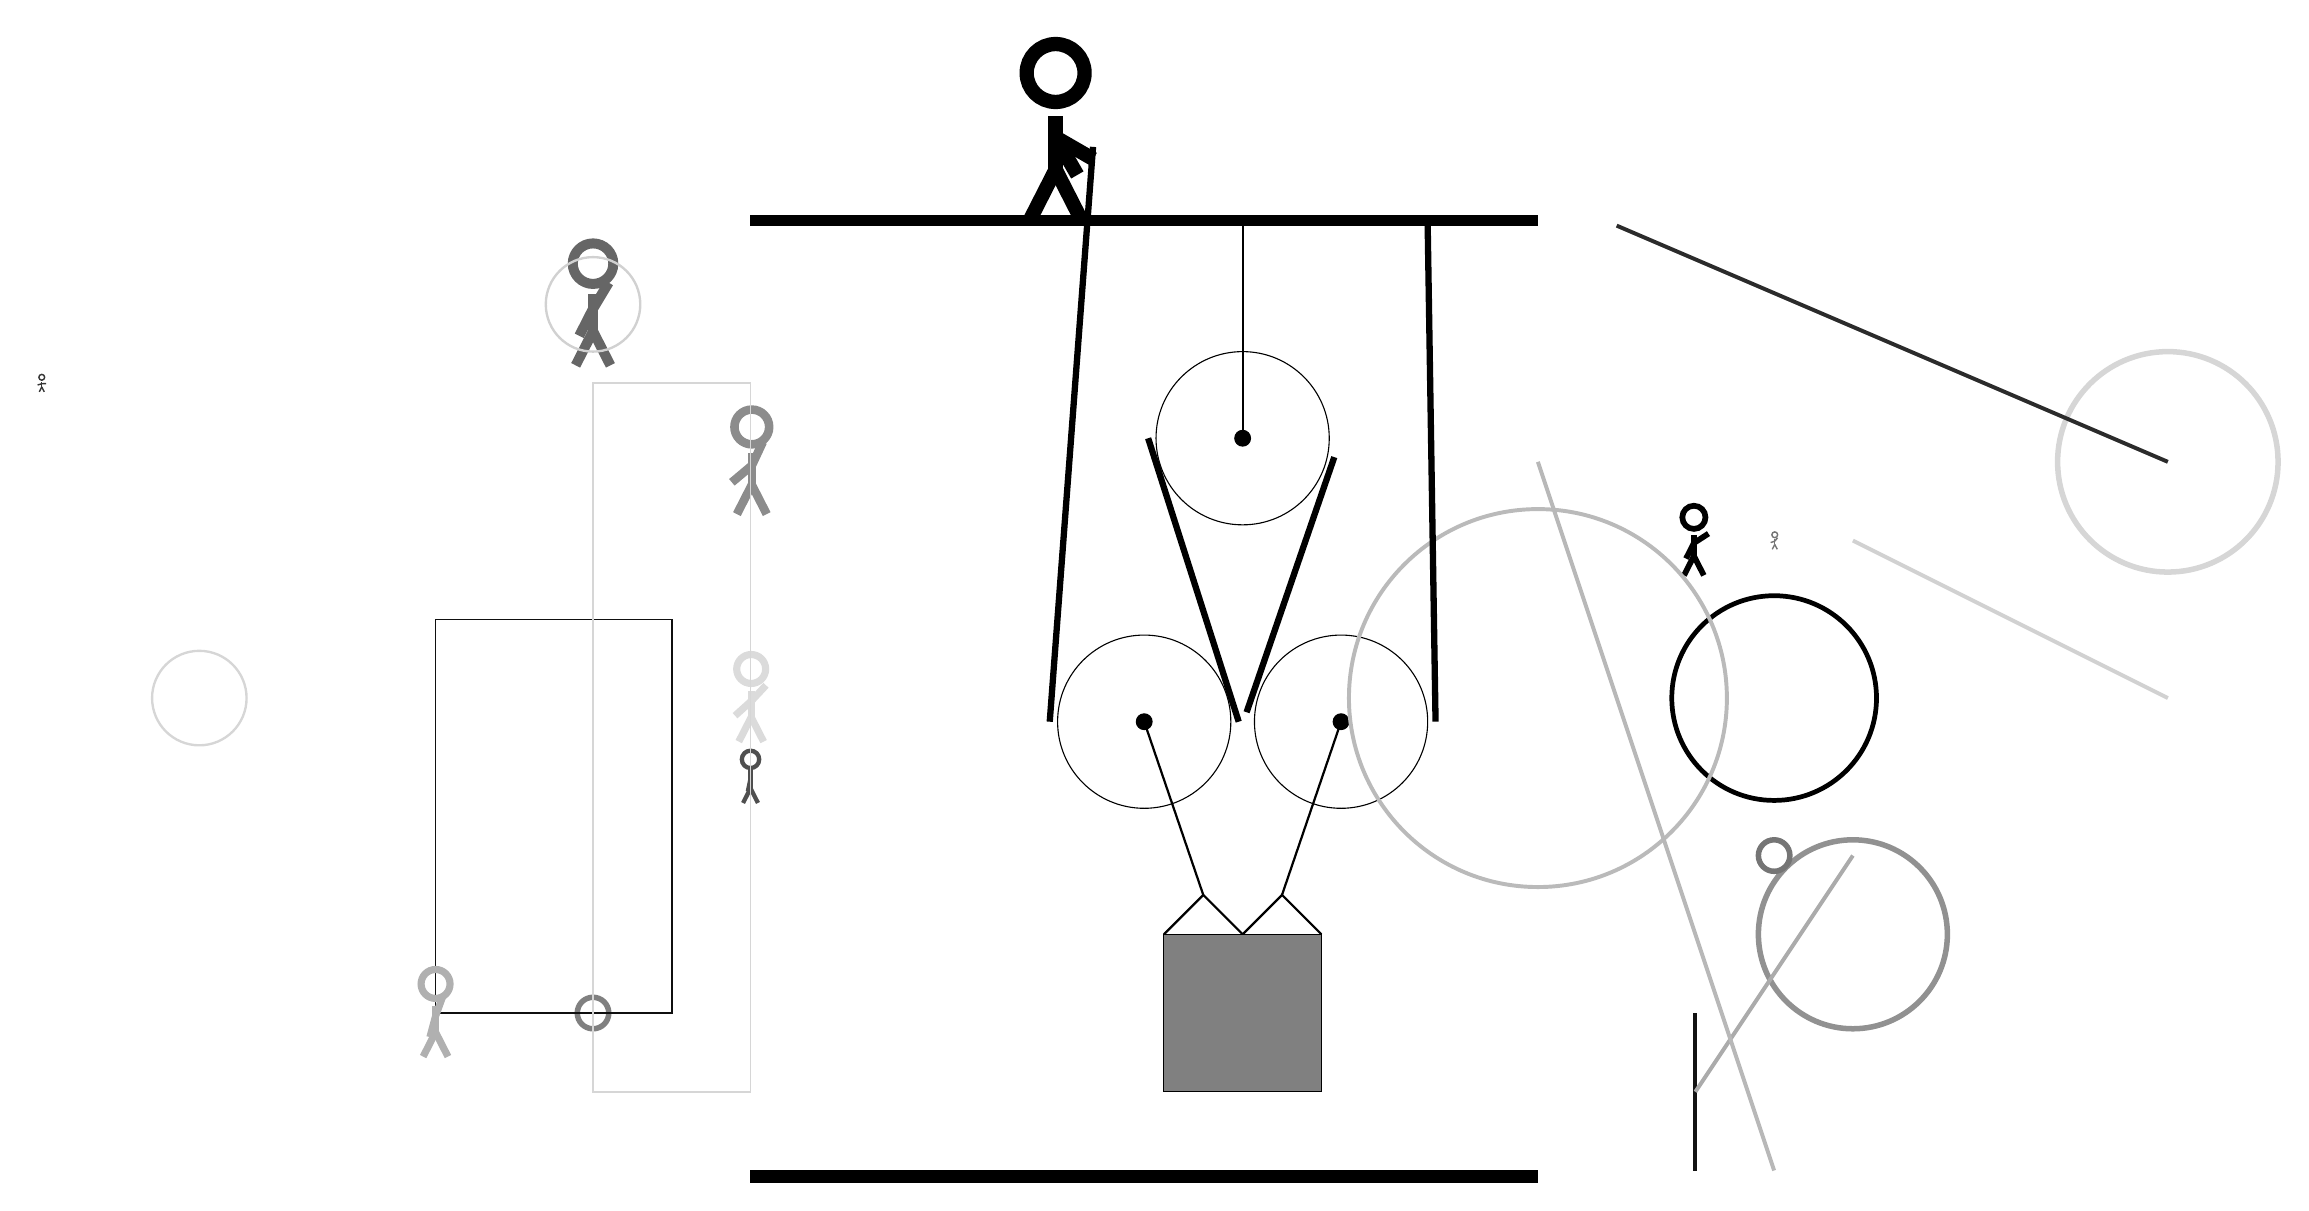
\begin{tikzpicture}
			%%%%% START %%%%%
			
			\draw[fill=black] (-4, 9) rectangle (6, 9.125);
			
			\draw (1, 2.7) circle (1.1);
			\draw[fill=black] (1, 2.7) circle (0.1);
			
			\draw (2.25, 6.3) circle (1.1);
			\draw[fill=black] (2.25, 6.3) circle (0.1);
			\draw[thick] (2.25, 6.3) -- (2.25, 9);
			
			\draw (3.5, 2.7) circle (1.1);
			\draw[fill=black] (3.5, 2.7) circle (0.1);
			
			\draw[thick] (3.5, 2.7) -- (2.75, 0.5);
			\draw[thick] (1, 2.7) -- (1.75, 0.5);
			\draw[thick]  (1.25, 0) -- (1.75, 0.5) -- (2.25, 0);
			\draw[thick]  (2.25, 0) -- (2.75, 0.5) -- (3.25, 0);
			\draw[fill=black!50] (1.25, 0) rectangle (3.25, -2);
			
			\draw [line width=0.7mm, color=black!16](14, 6) circle (1.4);
			
			\draw [line width=0.7mm, color=black!50](-6, -1) circle (0.2);
			\node[line width=0.3mm, color=black!79] at (-13, 7) {\Strichmaxerl[1][17][1]};
			\draw[line width=0.2mm, color=black!94] (-5, 4) rectangle (-8, -1);
			\draw [line width=0.7mm, color=black!43](10, 0) circle (1.2);
			\node[line width=0.2mm, color=black!100] at (8, 5) {\Strichmaxerl[4][63][33]};
			
			\node[line width=0.7mm, color=black!69] at (-4, 2) {\Strichmaxerl[3][78][90]};
			
			\draw[line width=0.5mm, color=black!93](8, -1) -- (8, -3);
			\node[line width=0.6mm, color=black!45] at (-4, 6) {\Strichmaxerl[6][40][65]};
			\draw[line width=0.5mm, color=black!18](10, 5) -- (14, 3);
			\node[line width=0.2mm, color=black!14] at (-4, 3) {\Strichmaxerl[5][42][47]};
			\draw [line width=0.6mm, color=black!100](9, 3) circle (1.3);
			\draw [line width=0.7mm, color=black!54](9, 1) circle (0.2);
			\draw [line width=0.5mm, color=black!27](6, 3) circle (2.4);
			\draw[line width=0.5mm, color=black!33](10, 1) -- (8, -2);
			\draw [line width=0.3mm, color=black!16](-11, 3) circle (0.6);
			\draw[line width=0.5mm, color=black!28](6, 6) -- (9, -3);
			\draw[line width=0.2mm, color=black!16] (-6, 7) rectangle (-4, -2);
			\node[line width=0.6mm, color=black!60] at (-6, 8) {\Strichmaxerl[7][63][59]};
			\draw [line width=0.3mm, color=black!18](-6, 8) circle (0.6);
			\node[line width=0.7mm, color=black!54] at (9, 5) {\Strichmaxerl[1][18][51]};
			
			\draw[line width=0.5mm, color=black!83](7, 9) -- (14, 6);
			
			\node[line width=0.5mm, color=black!31] at (-8, -1) {\Strichmaxerl[5][75][70]};
			
			\draw[line width=0.8mm] (0.35, 10) --  (-0.2, 2.7);
			\centerarc[line width=0.8mm](1, 2.7)(180:360:1.2000000000000002);
			\draw[line width=0.8mm] (2.2, 2.7) -- (1.05, 6.3);
			\centerarc[line width=0.8mm](2.25, 6.3)(-20:180:1.2000000000000002);
			\draw[line width=0.8mm](3.414, 6.06) -- (2.3, 2.82);
			\centerarc[line width=0.8mm](3.5, 2.7)(160:360:1.2000000000000002);
			\draw[line width=0.8mm](4.7, 2.7) -- (4.6, 9);
			
			\node at (-0.07, 10.2) {\Strichmaxerl[10][120][-30]};
			
			\draw[fill=black] (-4, -3) rectangle (6, -3.15);
			
			%%%%% END %%%%%
		\end{tikzpicture}
	\end{figure}	
\end{document}